%%%%%%%%%%%%%%%%%%%%%%%%%%%%%%%%%%%%%%%%%%%%%%%%%%%%%%%%%%%%%%%%%%%%%%
%%                     Logic arc
%%%%%%%%%%%%%%%%%%%%%%%%%%%%%%%%%%%%%%%%%%%%%%%%%%%%%%%%%%%%%%%%%%%%%%
%\color{blue}
\subsection{Glyph: \glyph{Logic arc} }\label{sec:logicArc}

\glyph{Logic arc} is used to represent the fact that an interactor influences
the outcome of a logic operator. 

\begin{glyphDescription}
 \glyphSboTerm SBO:0000398 - logical relationship.
 \glyphOrigin Any \glyph{interactor} (\sect{interactors}) or \glyph{logical operator} (\sect{logic}).
 \glyphTarget Any \glyph{logical operator} (\sect{logic}).
 \glyphEndPoint No particular symbol is used to represent a logic arc.
 \end{glyphDescription}

% Change the image to fit ER and not PD

\begin{figure}[H]
  \centering
  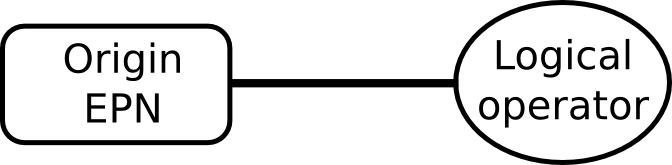
\includegraphics[scale = 0.4]{images/logicArc}
  \caption{The \ER glyph for \glyph{logic arc}.}
  \label{fig:logicArc}
\end{figure}
